\section{Models and Methods}
\label{sec:methods}

This section describes the two dynamical systems we assimilate, the full
4D-Var cost we minimize, the learned inverse
observation operator and its two convolutional variants, our observation-noise
model, the correlation preconditioning, the optimizer, and the sliding-window
cycling scheme. Throughout, $\Mop^t(\xstate_0)$ denotes the model state at
outer step $t$ integrated from the initial condition $\xstate_0$, $\Hop$ is the
(sparse, subsampling) observation operator, and $\yobs_t = \Hop\Mop^t(\xstate_0)
+ \boldsymbol\varepsilon_t$ the corresponding noisy observation.

\subsection{Dynamical systems}

The first testbed is the 1D Lorenz-96 model
\citep{lorenz1996predictability}, a periodic chain of $K=40$ grid points
evolving under the ordinary differential equation (ODE)
\begin{equation}
\dot{x}_k = (x_{k+1}-x_{k-2})\,x_{k-1} - x_k + F,
\qquad x_{k+K}=x_k,
\label{eq:l96}
\end{equation}
with forcing $F=8$ and cyclic indices. We integrate
Eq.~\eqref{eq:l96} with a hand-written fixed-step fourth-order Runge--Kutta
(RK4) scheme in which each outer step $\Delta t = 0.1$ MTU is
composed of ten inner RK4 substeps of size $0.01$. The observation operator
$\Hop$ subsamples every fourth grid point, so the $40$-dimensional state is
observed at only $10$ sites.

To check that this fixed-step integrator is faithful at the short horizons
relevant to assimilation, we compared it against an adaptive Dormand--Prince
(dopri5) solver \citep{dormand1980family}. Starting from identical attractor
states, the $L^2$ trajectory divergence stays near machine precision while
$t \ll T_L$ and first reaches the order-one (state-norm) scale at a median
$t^{\star}=7.70$ MTU (range $[6.50,8.30]$ over five warmed-up states; $6.30$ MTU
for a single trajectory), saturating near $28.5$ once the trajectories fully
decorrelate by $t\approx 19.9$ MTU. A direct two-trajectory separation fit
(initial separation $10^{-6}$, fitted over $t\in[0.5,5.0]$ MTU) gives a leading
exponent $\lambda = 2.263\,\mathrm{MTU}^{-1}$ and a Lyapunov time
$T_L = 1/\lambda = 0.442$ MTU. This is shorter than the value of $\sim 0.6$ MTU
expected from the literature, a known consequence of the coarse fixed-step
integrator that we report honestly; our single-window experiments use a window
of $T=10$ outer steps ($1.0$ MTU), comfortably inside $t^{\star}$, so this
integrator choice does not contaminate the assimilation results.

The second testbed is 2D Kolmogorov flow: the vorticity form
of the incompressible Navier--Stokes equations (a partial differential
equation, PDE) on the periodic domain $[0,2\pi]^2$ with sinusoidal Kolmogorov
forcing at wavenumber $k=4$, viscosity $\nu=10^{-2}$, and linear (Rayleigh)
drag $\alpha=0.1$, following the solver design of \citet{kochkov2021machine}.
The state is a single vorticity field $\omega$ on a $64\times 64$ grid
($4096$ degrees of freedom), advanced with a pseudo-spectral RK4 solver at outer
step $0.18$ composed of $25$ inner substeps. Here $\Hop$ subsamples every
sixteenth point in each direction, giving a $4\times 4$ observation grid
($16$ of $4096$ points observed). Warmed-up initial conditions are produced by
integrating a spectrally filtered random field forward $100$ outer steps; a
warmup diagnostic confirms the flow reaches a statistically stationary
turbulent regime, with the enstrophy $\tfrac12\langle\omega^2\rangle$ rising
from $0.50$ at the smooth cold start to $\approx 9.8$ near the warmup horizon
(last-$20$-step relative drift $\approx 10.8\%$, i.e.\ approximately
quasi-stationary) and the training-trajectory vorticity spanning roughly
$[-12.3,14.1]$.

\subsection{Observation-noise model}

Departing from the original study, which assimilated clean observations, every
experiment here corrupts the observations with independent additive Gaussian
noise,
\begin{equation}
\yobs = \Hop(\xstate) + \boldsymbol\varepsilon,
\qquad
\boldsymbol\varepsilon \sim \mathcal{N}\!\left(\bm{0},\,\sigobs^2\bm{I}\right),
\label{eq:noise}
\end{equation}
applied independently at each observed site and time, so that the
observation-error covariance is $\Rcov = \sigobs^2\bm{I}$. For the Lorenz-96
single-window experiments we use $\sigobs \in \{0.1, 0.5, 1.0\}$, spanning a
range from a sharp, nearly-clean perturbation to a level comparable to the
Lorenz-96 state amplitude; Figure~\ref{fig:noisedist} plots the three
corresponding probability density functions. The sliding-window runs use
$\sigobs \in \{0.0, 0.5\}$ for Lorenz-96 and $\{0.0\}$ for Kolmogorov flow. In
the cost, $\sigobs$ doubles as the inverse-variance weight on the observation
term; the perfect-observation case is handled by flooring it (at $0.1$ for
Lorenz-96 and $0.05$ for Kolmogorov flow) so that $\Jo$ remains finite.

\begin{figure}[t]
  \centering
  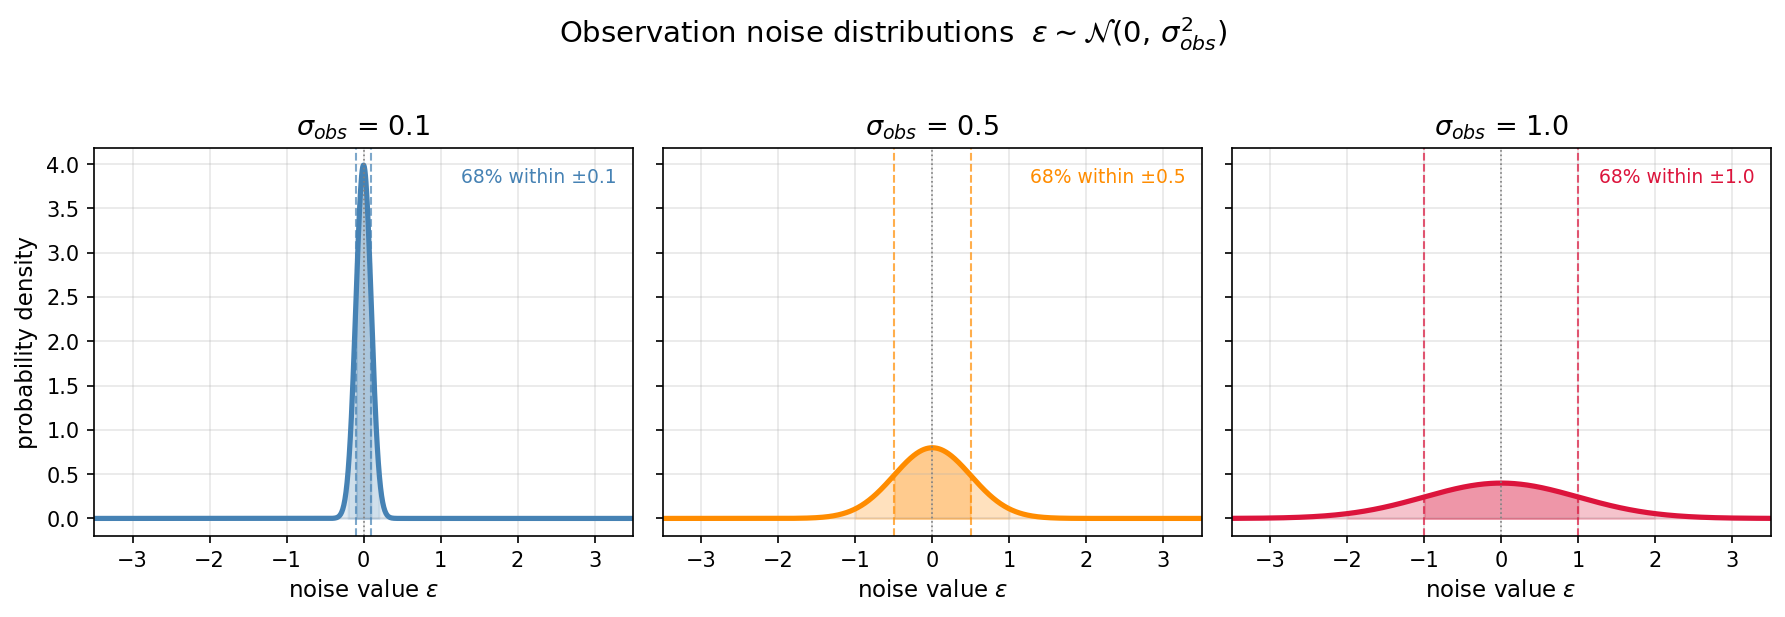
\includegraphics[width=0.95\linewidth]{noise_distributions.png}
  \caption{Gaussian observation-noise probability density functions used to
  corrupt the observations in every experiment. Each curve is the density of
  $\varepsilon \sim \mathcal{N}(0, \sigobs^2)$ for one of the three noise
  standard deviations $\sigobs \in \{0.1, 0.5, 1.0\}$; the horizontal axis is
  the noise value added to a single observed component and the vertical axis is
  the probability density. Each observed site and time receives an independent
  draw, so the observation-error covariance is $\Rcov = \sigobs^2 \bm{I}$. The
  $\sigobs=0.1$ case is a sharp, nearly-clean perturbation, whereas
  $\sigobs=1.0$ broadens to a level comparable to the Lorenz-96 state amplitude,
  making observations substantially less informative and stress-testing the
  assimilation methods.}
  \label{fig:noisedist}
\end{figure}

\subsection{The full 4D-Var cost}

Our central extension replaces the paper's bare observation-misfit objective
with the complete 4D-Var cost \citep{ledimet1986variational,courtier1994strategy},
$J(\xstate_0) = \Jb + \Jo$, where
\begin{equation}
J(\xstate_0)
= \underbrace{\tfrac12 (\xstate_0-\xstate_b)^{\top}\Bcov^{-1}(\xstate_0-\xstate_b)}_{\Jb}
+ \underbrace{\tfrac12 \sum_{t}\,(\Hop\Mop^t(\xstate_0)-\yobs_t)^{\top}\Rcov^{-1}(\Hop\Mop^t(\xstate_0)-\yobs_t)}_{\Jo},
\label{eq:4dvar}
\end{equation}
with background covariance $\Bcov = \sigb^2\bm{C}$ ($\bm{C}$ the spatial
correlation), observation-error covariance $\Rcov = \sigobs^2\bm{I}$, and
$\xstate_b$ the background (prior) estimate. The background term $\Jb$ pulls the
analysis toward $\xstate_b$ and is what makes the problem well-posed when
observations are sparse ($10$ of $40$ for Lorenz-96, $16$ of $4096$ for
Kolmogorov flow); $\sigb$ is the background-error standard deviation we tune.

\paragraph{Decorrelation preconditioning (Lorenz-96 only).}
We estimate $\bm{C}$ as the spatial covariance of an ensemble of warmed-up
states (condition number $8.72$, climatological mean $\approx 2.34$) and optimize
in decorrelated coordinates $\bm{z}=\bm{C}^{-1/2}\xstate$, obtained from a
symmetric eigendecomposition. With $\Bcov=\sigb^2\bm{C}$ this reduces the
background term to the isotropic
$\Jb = \lVert\bm{z}_0-\bm{z}_b\rVert^2/(2\sigb^2)$; the starting point is
decorrelated before optimization and the optimized $\bm{z}_0$ is re-correlated
to physics coordinates at the end. For Kolmogorov flow we instead optimize the
vorticity field directly with an identity background, $\Bcov=\sigb^2\bm{I}$ and
$\Jb=\lVert\omega_0-\omega_b\rVert^2/(2\sigb^2)$, because forming and factorizing
a full $4096\times 4096$ spatial covariance is prohibitively expensive.

\subsection{Learned inverse observation operator}

Following the paper's key idea, we train a CNN
$\Hinv$ that acts as a learned inverse observation operator, mapping a stacked
(time, space) tensor formed from an observation sequence $Y\in\mathbb{R}^{T\times
n_{\text{obs}}}$ back to a full-state sequence $X\in\mathbb{R}^{T\times
n_{\text{grid}}}$. Its building block is a periodic-space convolution: the
spatial axis receives \emph{circular} padding (matching the periodic boundary
conditions) while the time axis receives \emph{zero} padding, after which the
low-resolution observation grid is upsampled to the full grid.

We implement two PyTorch \citep{paszke2019pytorch} variants. The
\emph{original-port} inverter uses a hidden width of $32$ over six residual
periodic-convolution blocks with Gaussian error linear unit (GELU) activations
and bilinear spatial upsampling. The \emph{paper-faithful} inverter follows the
architecture of \citet{frerix2021invobs} more closely: sigmoid linear unit
(SiLU) activations \citep{elfwing2018sigmoid}, batch normalization (BN) after
every convolution \citep{ioffe2015batch}, cubic periodic upsampling, and a
decreasing channel pyramid of widths $128/64/32/16$ with no skip connections.
Both are trained by supervised regression --- integrate trajectories, apply
$\Hop$ (plus noise), and fit the network to recover the full state under a
mean-squared-error (MSE) loss with the Adam optimizer. Trained at $\sigobs=0$ on
$32{,}000$ Lorenz-96 trajectories, the two variants reach comparable
reconstruction quality (held-out test $L_1$ ratio $1.165$), and the
paper-faithful inverter is retrained at each noise level to supply a
noise-matched lift for the hybrid runs.

\paragraph{Physics-space hybrid companion cost.}
The learned inverse enables a second, more nearly convex objective that
replaces the lossy observation misfit $\Jo$ with a full-state misfit against the
lifted observations,
\begin{equation}
J_{\text{phys}}(\xstate_0)
= \Jb + \frac{1}{2\sigma_p^2}\sum_t \big\lVert \Mop^t(\xstate_0) - [\Hinv(Y)]_t \big\rVert^2,
\label{eq:physcost}
\end{equation}
where $\Hinv(Y)$ lifts the observation sequence into physics space, removing the
many-to-one operator $\Hop$ from inside the objective. The \emph{hybrid}
schedule runs physics-space optimization first as a warm start
(Eq.~\eqref{eq:physcost}) and then refines against the true observations with the
observation-space cost $\Jb+\Jo$ (Eq.~\eqref{eq:4dvar}); we contrast it
throughout against pure observation-space optimization. The learned operator is
also used as an initializer: the cold-start guess $\Hinv(Y)$ replaces a naive
interpolation or climatological-mean baseline.

\subsection{Optimization}

All variational sub-problems are solved with the L-BFGS quasi-Newton method
\citep{liu1989limited} using a strong-Wolfe line search. The entire
$N$-sample ensemble is optimized in a single batched L-BFGS call: because each
row's gradient depends only on its own observations, the batched problem is
exactly equivalent to $N$ independent 4D-Var problems. The hybrid schedule
allocates a fixed number of physics-space iterations followed by
observation-space iterations (for Lorenz-96 cycling, $100$ then $400$), whereas
pure observation-space runs spend the full iteration budget on $\Jb+\Jo$.

\subsection{Sliding-window (cycling) 4D-Var}

We extend the single-window setup to an operational cycling scheme. A
fixed-length assimilation window (Lorenz-96 \texttt{WINDOW\_T}$=8$; Kolmogorov
\texttt{WINDOW\_T}$=10$ outer steps) slides over a long observation record with a
configurable \emph{stride} controlling window overlap (Lorenz-96 strides
$\{2,4,8\}$ for $T_{\text{obs}}\in\{24,48\}$; Kolmogorov strides $\{2,5,10\}$ for
$T_{\text{obs}}\in\{20,30\}$). The two roles of the background are decoupled: on
cycle $0$ the $\Jb$ background equals the cold-start initializer, while for
cycles $\ge 1$ the background is the \emph{propagated previous analysis} --- the
prior cycle's optimized state integrated forward to the new window start. Each
cycle re-initializes the L-BFGS starting point from a fresh $\Hinv$ estimate of
the current window, and the noise-matched inverter checkpoint is used at each
cycle. The stride is chosen so that the most recent window is always assimilated
even when $(T_{\text{obs}}-\texttt{WINDOW\_T})$ is not divisible by it. Because
cycling trusts the propagated analysis, it uses a tighter background variance
($\sigb=0.3$) than the cold-start single window ($\sigb=1.0$).
